% Set the author and title of the compiled pdf
\hypersetup{
  pdftitle = {\Title},
  pdfauthor = {\Author}
}

\definecolor{mygreen}{rgb}{0,0.6,0}
\definecolor{mygray}{rgb}{0.5,0.5,0.5}
\definecolor{mymauve}{rgb}{0.58,0,0.82}

\lstset{ %
  backgroundcolor=\color{white},   % choose the background color; you must add \usepackage{color} or \usepackage{xcolor}
  basicstyle=\footnotesize,        % the size of the fonts that are used for the code
  breakatwhitespace=false,         % sets if automatic breaks should only happen at whitespace
  breaklines=true,                 % sets automatic line breaking
  captionpos=b,                    % sets the caption-position to bottom
  commentstyle=\color{mygreen},    % comment style
  deletekeywords={...},            % if you want to delete keywords from the given language
  escapeinside={\%*}{*)},          % if you want to add LaTeX within your code
  extendedchars=true,              % lets you use non-ASCII characters; for 8-bits encodings only, does not work with UTF-8
  frame=single,                    % adds a frame around the code
  keepspaces=true,                 % keeps spaces in text, useful for keeping indentation of code (possibly needs columns=flexible)
  keywordstyle=\color{blue},       % keyword style
  language=Java,                 % the language of the code
  morekeywords={*,...},            % if you want to add more keywords to the set
  numbers=left,                    % where to put the line-numbers; possible values are (none, left, right)
  numbersep=5pt,                   % how far the line-numbers are from the code
  numberstyle=\tiny\color{mygray}, % the style that is used for the line-numbers
  rulecolor=\color{black},         % if not set, the frame-color may be changed on line-breaks within not-black text (e.g. comments (green here))
  showspaces=false,                % show spaces everywhere adding particular underscores; it overrides 'showstringspaces'
  showstringspaces=false,          % underline spaces within strings only
  showtabs=false,                  % show tabs within strings adding particular underscores
  stepnumber=1,                    % the step between two line-numbers. If it's 1, each line will be numbered
  stringstyle=\color{mymauve},     % string literal style
  tabsize=2,                       % sets default tabsize to 2 spaces
  title=\lstname                   % show the filename of files included with \lstinputlisting; also try caption instead of title
}

\section{Algorithmic complexity and performance}

Algorithmic complexity and the big-oh notation allows us to characterise the
time and space requirements of an algorithm when it is given varying input data.
The big-oh notation allows us to get a good approximation of the upper and lower
bounds of an algorithm's complexity.

We can work out such an approximation by analysing (and generalising) the number
of logical operations an algorithm might do, rather than inspecting it's
performance in an implementation. This allows us to compare the merits of
different algorithms irrespective of their implementation.

The big-oh notation is shown below:

\[
  O(growth rate)
\]

The growth rate represents the rate at which the complexity of the algorithm
will change with the size of the input.

Growth rates that are either exponential or factorial in nature (or are perhaps
even worse than this) are said to be intractable \marginpar{Tractable
(\textit{Adjective})\\Easy to deal with.}, while algorithms with other
computational complexities are said to be tractable.

\newcommand\multibrace[3]{\rdelim\}{#1}{3mm}[\pbox{#2}{#3}]}

\begin{table}[h!]
  \centering
  \begin{tabularx}{0.75\textwidth}{>{$}l<{$} l l}
    \text{Complexity} & Growth rate \\ \cline{1-2}
    O(1)              & None\\
    O(log n)          & Logarithmic\\
    O(n^k)            & Polynomial\\
    O(n)              & Linear & \multibrace{3}{4.6cm}{
                                  All of these are special cases of polynomials,
                                  $n^1, n^2$ and $n^3$ respectively
                                } \\
    O(n^2)            & Quadratic\\
    O(n^3)            & Cubic\\
    O(k^n)            & Exponential\\
    O(n!)             & Factorial\\
  \end{tabularx}
  \caption{A number of common complexities and their equivalent growth rates}
  \label{table:complexity}
\end{table}

\subsection{Simplifying Big-Oh expressions}

In order to simplify the big-oh complexity of an algorithm you just isolate the
fastest growing term in the equation (i.e. whatever term comes furthest down in
Table~\ref{table:complexity}). You then remove all the constants from the
equation.

For example, given $O(2n + 1)$, this simplifies to $O(n)$ since constant terms
are taken out. $O(n + n^2)$ simplifies to $O(n^2)$ since smaller terms are taken
out when they are added. Note that if terms are multiplied together, they are not
simplified e.g. $O(n \times \log n)$, stays as $O(n\log n)$.

\subsection{Analysing algorithmic complexity}

There are two ways of finding the complexity of an algorithm, to inspect the
psudo code for it, or by implementing the algorithm and experimentally
determining the change in it's runtime with different input sizes.

\marginpar{Remember to check that your psudo code correctly implements the
algorithm before you try this.}

In order to analyse the psudo code to work out the complexity, you must look at
how many primitive operations it will use for different sizes of input.
Primitive operations are defined as memory accesses, arithmetic operations,
comparisons and the like.

As a general rule, loops, recursion and other constructs for repeatedly
performing operations will be the best indicator as to the complexity of
algorithms.

If an algorithm is reducing the data it has to work with every so often, then it
may have a logarithmic runtime. For example, if an algorithm utilises a binary
chop (such as binary search), then its runtime probably has a $log_2$ inside.
See section~\ref{subsubsec:logs} for a bit more on logs.

In order to determine complexity experimentally, you must implement the
algorithm in a programming language of your choice, then run the program for
different input sizes and measure the runtime and the memory used. Plot the data
on a graph and extrapolate as needed. From the curve of the graph, it is
possible to predict the complexity of the algorithm.

\subsubsection{A refresher on logs}
\label{subsubsec:logs}

A logarithm of a number is the exponent to which another number (the base) must
be raised to produce that number:

\begin{gather*}
  \forall b,x,y \in \mathbb{Z}\\
  y = b^x \Leftrightarrow x = log_b(y)
\end{gather*}

Henceforth, $2^4 = 16$ and $log_2(16) = 4$.

\subsubsection{Finding the maximum input size}

If we know the complexity and running space/time of an algorithm for a specific
implementation and input, we might want to know the input size we could run the
algorithm with for the specific machine in a specific time, or within a specific
space limit.

The way you do this is by solving the big-oh equation for $t$ instead of $n$.
For example, if the algorithm takes $30$ seconds to process $1000$ kilobytes of
data, how long will it take if we double the processing speed, given that the
algorithm runs in $O(n^3)$ time?

%TODO: Work out if this is BS or not?

\begin{gather*}
  t = n^3\\
  \sqrt[\leftroot{-0}\uproot{3}3]{t} = n\\
  \text{When we double $n$ and $t$:}\\
  2n = \sqrt[\leftroot{-0}\uproot{3}3]{2t}\\
  2n = 1.25992104989t\\
  30 / 1.25992104989 \approx 24\\
\end{gather*}

\subsection{The master theorem}

\marginpar{See pages 268-270 in the course textbook for more information}

The master method is a way of solving divide and conquer recurrence equations
without having to explicitly use induction. It is used when an algorithm's
complexity is of the form:

\[
  T(n) = 
  \begin{cases}
    c               & \text{if $n \le d$}\\
    aT(n/b) + f(n)  & \text{if $n \geq d$}
  \end{cases}
\]

Where $f(n)$ is a function that is positive when $n \geq d$ and:

\begin{tabular}{>{$}l<{$}}
  d \geq 1\\
  a > 0\\
  b > 1\\
  c > 0\\
  d \in \mathbb{Z}\\
  a,b,c \in \mathbb{R}
\end{tabular}

Such a recurrence relation occurs whenever an algorithm uses a divide and
conquer approach. Such an algorithm will split the problem into $a$ subproblems,
each of size $n/b$ before recursively solving them and merging the result back
together. In this case, $f(n)$ is the time it takes to split the problem into
subproblems and merge them back together after the solving is done.

There is more after this, that I don't understand. Check out the textbook, or
the internet...

%The master theorem is defined by three cases:

%\begin{enumerate}
%  \item If there is a small constant $\epsilon > 0$ such that $f(n)$ is
%        $O(n^{log_{b}{a-\epsilon}})$, then $T(n)$ is $\Theta(n^{log_ba})$
%
%        An example could be when the recurrence relation is
%        \[
%          T(n) = 4T(n/2) + n
%        \]
%        since $n^{log_{b}{a}} = n^{log_{2}{4}} = n^2$, therefore $T(n) =
%        \Theta(n^{log_24}) = \Theta(n^2)$.
%  \item % TODO:
%        At this point I'm not sure what's going on...
%\end{enumerate}

\subsection{Amortized Analysis}

\begin{aquote}{Rebecca Fiebrink, Amortized Analysis Explained, Princeton University}
  Amortized analysis is a technique for analysing an algorithm's running time.
  It is often appropriate when one is interested in understanding asymptotic
  behaviour over sequences of operations. For example, one might be interested in
  reasoning about the running time for an arbitrary operation to insert an item
  into a binary search tree structure. In cases such as this, it might be
  straightforward to come up with an upper bound by, say, finding the
  worst possible time required for any operation, then multiplying this by the
  number of operations in the sequence. However, many real data structures, such
  as splay trees, have the property that it is impossible for every operation in
  a sequence to take the worstcase time, so this approach can result in a
  horribly pessimistic bound! With a bit of clever reasoning about properties of
  the problem and data structures involved, amortized analysis allows a tighter
  bound that better reflects performance.
\end{aquote}

The idea is based on the fact that some high cost operations may do lots of the
work for later operations, which means that these later operations are low cost.
In order to encapsulate this in our analysis, we need to come up with a
`potential' function that captures how operations with different costs affect
our datastructure.

\subsubsection{Aggregate analysis}

This is the most simple method of amortized analysis. You find a bound on the
sequence of operations, and then divide it by the number of operations to find
the amortized cost. This only works when all operations have the same cost, such
as pushing and popping items with a stack. If we want to push/pop $n$ items,
then the total cost would be $n$ (assuming is costs $1$ for each push or pop),
so the amortized cost would be $\frac{n}{n} = 1$.

\subsubsection{Banker's method}

This method takes the view that each operation has a predefined cost that must
be paid in order to execute it. You would need to insert coins into the computer
for each operation based on it's cost. The cost does not necessarily equate to
the complexity of the operation, in which case, any difference will be added to
(or subtracted from) a `bank account'.

This means that, operations that take a long time (say re-balancing a tree, or
an insert into a heap that requires a lot of re-organisation), will be able to
take money from the bank account in addition to their own fee in order to `pay'
for their time.

In this way, \textbf{the amount charged for each operation is the amortized cost
for that operation}.

The hard bit with this method is to pick appropriate costs for each operation
and show that they are sufficient to allow payment for any sequence of valid
operations. If $c_i$ is the actual cost of the $i$th operation, $C$ is the cost
we charge per operation, and if we do $n$ operations, then the following must
hold for us to always have a positive bank account:

\[
  \sum\limits_{i = 1}^nC \geq \sum\limits_{i=1}^nc_i
\]

In order to reason about never falling into debt with a negative bank balance,
it's a good idea to keep a track of which operations generated what credit, and
store it in different `sections' of the bank account. This could mean that each
position in a stack ends up with having a certain amount of credit associated
with it, or each node in a tree.

Lets analyse an extendable array. When it has reached it's limit, we create a
new array of double the length and copy the current one across.

If we set a cost of $3$ for every array write, then this should cover the cost
of copying when the size limit is reached. Note, that on `normal' writes (i.e.
where we don't have to resize the array), we will only add \textsterling$2$ to
the bank since \textsterling $1$ is taken up for the write operation. We start
with an empty array of size 0:

\begin{figure}[H]
  \centering
  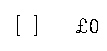
\includegraphics[height=15mm]{diagrams/banker0.pdf}
  \label{banker0}
\end{figure}

Now, lets add 1:

\begin{figure}[H]
  \centering
  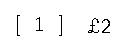
\includegraphics[height=15mm]{diagrams/banker1.pdf}
  \label{banker1}
\end{figure}

Now, in order to add 2, we'll need to resize the array, which costs
\textsterling 1 for copying the current item over, and then add the new 2 in, so
we'll use up \textsterling 2:

\begin{figure}[H]
  \centering
  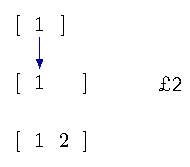
\includegraphics[height=50mm]{diagrams/banker2.pdf}
  \label{banker2}
\end{figure}

Now, in order to add 3, we'll need to resize the array, which costs
\textsterling 2 for copying the current ones over, and then add the new 3 in, so
we'll use up \textsterling 3:

\begin{figure}[H]
  \centering
  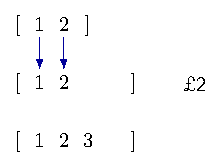
\includegraphics[height=50mm]{diagrams/banker3.pdf}
  \label{banker3}
\end{figure}

Adding 4 is normal:

\begin{figure}[H]
  \centering
  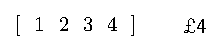
\includegraphics[height=15mm]{diagrams/banker4.pdf}
  \label{banker4}
\end{figure}

But to add 5, we need another resize, costing $4 + 1 = \text{\textsterling} 5$
(we also get an income of \textsterling 3 too though):

\begin{figure}[H]
  \centering
  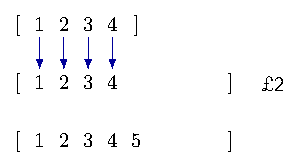
\includegraphics[height=50mm]{diagrams/banker5.pdf}
  \label{banker5}
\end{figure}

Lets whizz forward to inserting 9. By this point, we'll have \textsterling 8.
We need to expand \textsterling 8 doing copying, and another adding 9, but we
get an income of \textsterling 3, so we're left with \textsterling 2 again:

\marginpar{If you didn't quite understand this, then take a look at section
1.5.2 in the course reading (Algorithm Design by Goodrich and Tamassia). The
same example is in there, and they have editors who's job it is to make sure
there's not any mistakes... }

\begin{figure}[H]
  \centering
  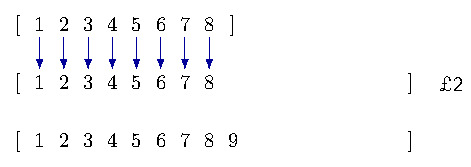
\includegraphics[height=50mm]{diagrams/banker9.pdf}
  \label{banker9}
\end{figure}

You can see here that we are able to maintain a resizable array by charging a
flat rate of \textsterling 3 on every insert. This means we can pay for the
insertion of $n$ elements into our array with $\textsterling 3n$, which means
our algorithm runs in $O(n)$ amortized time.

\subsubsection{Potential method}

\marginpar{The idea of `potential' comes from potential energy in physics, which
can be defined as ``The energy stored in a system due to it's configuration''.}

The potential method is similar to the banker's method in that it requires
virtual money for each operation and it keeps a bank account (of potential in
this case) with which to finance expensive operations, however, \textbf{in the
potential method, the amortized cost of the operation $i$ is equal to the actual
cost plus the increase in potential due to the operation}.

Mathematically, if we define $\Phi$ to be the potential function, which takes as
an argument, the datastructure $D$ at a specific state after the $i$th
operation, and $c_i$ to be the cost of operation $i$, then the cost of the
operation will be:

\[
  C = c_i + \left(\Phi(D_i) - \Phi(D_{i-1})\right)
\]

We can derive the following equation (I won't try to here):

\[
  \sum\limits_{i=1}^n C = \sum\limits_{i=1}^n \left( c_i \right) + \Phi(D_n) - \Phi(D_{0})
\]

If $\Phi(D_i) \geq \Phi(D_0)$ for all $i$, then we know we will never run out of
potential.

Lets say we have a stack structure, that implements \texttt{push} to push one
element, and \texttt{popNPush}, which pops $k$ elements, and pushes another. Our
potential function could be: 

\[
  \Phi(D_i) = \text{\textit{The number of items in the stack after operation $i$}}
\]

This means that \texttt{push} will always have a cost of:

\begin{align*}
  C_{\text{\texttt{push}}} &= 1 + \left(\Phi(D_i) - \Phi(D_{i-1})\right)\\
                           &= 1 + \text{\#items} + \text{\#items - 1}\\
                           &= 1 + 1\\
                           &= 2
\end{align*}

Lets work out the cost for \texttt{popNPush}:

\begin{align*}
  C_{\text{\texttt{popNPush(k)}}} &= (k + 1) + (n - k + 1) - n\\
                                  &= 2 + k - k + n - n\\
                                  &= 2
\end{align*}

We can conclude that the total amortized cost for both \texttt{push} and
\texttt{popNPush} is $2$, so they have a amortized running time of $O(1)$.

\subsubsection{Comparing the banker's and the potential methods}

The banker method focuses on each operations prepayment by charging each
operation a fixed sum according to it's type, which will offset future expensive
operations made possible by this operation. The potential method focuses on the
current operation, and how it affects the datastructure/system now, and the
corresponding change in opportunity for future operations.

Often, the banker method will store credit throughout the datastructure/system,
maybe assigning each stack frame some credit, or maybe putting it in the
branches of a tree. In contrast, the potential method takes a more holistic view
and analyses the datastructure/system as a whole, maybe asking, how deep is the
stack, or what is the depth of the tree.

It is harder to come up with a decent cost function $\Phi$ in the potential
method than it is to work out the cost of operations in the banker method, but
for the potential method, you only have to do it once, whilst in the banker
method, you have to do it for each possible operation.

\section{Basic algorithms}

\subsection{Sorting}

A sorting algorithm takes as an input, an array of keys, where there is a
\textit{total order} on the keys (each key can be compared to another), and
produces as an output, the array where the keys are ordered according to their
order.

A total order is a relation that is transitive ($a \leq b \wedge b \leq c
\implies a \leq c$), anti-symmetric ($a \leq b \wedge b \leq a \implies a = b$),
and unsurprisingly, total $\neg(a \leq b \Leftrightarrow b \leq a)$.

If the ordering on the elements of the array isn't a total order then bad things
can happen when you try and use an algorithm to sort the data. For example, if
you were to try and sort an array of rocks, papers and scissors according to the
rules of the traditional game, then you wouldn't have a transitive relation, and
a (comparison based) sorting algorithm would probably loop infinitely.

\subsection{The complexity of sorting}

The most common sorting algorithms are $O(n^2)$ time (this includes $O(n
\log{n})$ algorithms too). Even though a polynomial sort time is good, sometimes
we have billions of items to sort, and henceforth, a very long running time. In
this situation, $n \log{n}$ sorts are much more preferable to $n^2$ sorts.

Since we often don't know in advance exactly what data any sorting function will
be given in advance, its important to know both the upper and lower bounds on
the complexity of the sorting algorithm we're using.

\begin{description}
  \item The \textbf{upper bound} is the worst case time complexity of the
  sort. For example the worst case complexity of Merge Sort is $O(n \log{n})$.

  \item The \textbf{lower bound} complexity is always at least $O(n)$ for
  sorting algorithms, since every item needs to be looked at once (if only to
  check that the list is already sorted). Bucket, radix and bubble sort all
  achieve this for certain inputs. No comparison based sort can ever achieve
  a lower bound with less than $O(log_2(n!)) \equiv O(n\log_2{n})$ comparisons.
\end{description}

\subsubsection{Worst case for comparison sorts}

If we were to draw a decision tree for each possible path of a comparison sort,
then we would get one with a depth of $log_2(n!)$, that produced all $n!$
permutations of the input. An asymptotically optimal comparison sort must travel
down this tree in its quest to find the answer. MergeSort and HeapSort are
optimal, while QuickSort is optimal for most inputs.

\subsection{Sorting algorithms in detail}
\begin{description}
\item \textbf{QuickSort} \\
  QuickSort is a \textbf{divide and conquer} algorithm, that uses a
  \textbf{comparison based} method to sort items. QuickSort can be implemented
  as an \textbf{in-place} sort, \textbf{stable}, though it is usually done so
  with recursion which gives it a space complexity of at least $O(log(n))$. This
  is a small inconvenience really though.

  First the list is partitioned into two halves. To do this, a random pivot is
  chosen from the list, and of the two new lists, one has the items less than
  the pivot, and the other has the items greater or equal to it.

  QuickSort is then applied to each sublist, so make them sorted, and then the
  start of the right list is joined to the end of the left list.

  See Listing~\ref{quicksort} for an example implementation.

\item \textbf{MergeSort} \\
  MergeSort is another \textbf{divide and conquer} algorithm that also uses a
  \textbf{comparison based} approach. MergeSort can \textbf{not be implemented
  in place}, but it is \textbf{stable}.

  It is similar to quicksort, except it's worst case run time is $O(n\log{n})$.
  First the list is split down the middle, and the two halves are sorted using
  merge sort recursively. Then, the two lists are merged back into one sorted
  list in $O(n)$ time. See Listing~\ref{mergesort} for an implementation.

\item \textbf{BucketSort} \\
  BucketSort is a \textbf{stable}, \textbf{distribution based} sorting
  algorithm. You place elements into `buckets' that describe a class of objects
  (you could order people by the first letter of their first name for example).
  When you've done that, you can either sort each bucket (using a different
  algorithm), then you simply return each bucket in order.

  BucketSort has a complexity of $O(n + k)$ where $k$ is the number of buckets
  you have. In the person name example, the number of buckets would be $26$,
  which, depending on the size of $n$ could be a very large, or very small
  factor.

\item \textbf{RadixSort}\\
  A RadixSort is basically bucket sort with multiple iterations. When you have
  sorted the first digit/word etc, you condense the buckets back into a list
  and, you apply the same sort again, except sorting on the second item.
  This repeats until you've sorted every character.digit in the list. RadixSort
  has a time complexity of $O(n)$, and is not in place.

  RadixSort can be done \textbf{in-place}, and in a \textbf{stable} manner:
  \begin{Verbatim}[commandchars=\\\{\},codes={\catcode`$=3\catcode`_=8}]
    050, 731, 806, 014, 235
    05\textbf{0}, 73\textbf{1}, 01\textbf{4}, 23\textbf{5}, 80\textbf{6}
    8\textbf{0}6, 0\textbf{1}4, 7\textbf{3}1, 2\textbf{3}5, 0\textbf{5}0
    \textbf{0}14, \textbf{0}50, \textbf{2}35, \textbf{7}31, \textbf{8}06
  \end{Verbatim}

\item \textbf{HeapSort} \\
  HeapSort is very simple, it iterates through the unsorted list, adding each
  element to a heap as it goes. When it has finished adding all the elements, it
  simply iterates through the heap and returns the order of iteration. Since
  adding an element to a (binary) heap is an $O(log(n))$ operation, and you need
  to do it $n$ times, the runtime of HeapSort is $O(n\log{n})$.

  HeapSort can be implemented \textbf{in place} since the heap can be stored
  inside the input array (since a heap can be represented as an array). HeapSort
  isn't stable though, since the heap can be re-ordered while it's being created
  (if you're not sure on this, maybe it's time for a trip to wikipedia to learn
  about heaps).

\end{description}

\subsection{Searching}

Searching algorithms are just as important as sorting algorithms, often partly
because they can be implemented to run in much less time and space.

\subsubsection{QuickSelect}
\label{QuickSelect}

QuickSelect is a cousin of QuickSort, designed to find the $k$th smallest
element in an unordered list. It's worst case performance is $O(n^2)$, but it's
average and best case is $O(n)$.

QuickSelect chooses an element as a pivot, and partitions the data into two
halves (elements less than, and elements greater or equal to the pivot).
QuickSelect then recurses only into the side that contains the element to be
found.

QuickSelect is usually implemented \textbf{in-place}, and if this is the case,
then a side effect of running QuickSelect will also partially sort the data.
QuickSelect can be implemented using tail recursion, and so it can use $O(n)$
memory space.

The main factor in the runtime of QuickSelect is the choice of pivot. If we
chose a pivot that decreased the list by the same fraction every time, then we
would get linear performance, but if we chose one that only decreased the list
by one every time, then we would get quadratic performance. Because of this, the
choice of pivot is very important. It is important to note that (just like
QuickSort) some inputs can be crafted to exhibit worst-case performance in
QuickSelect, which can have security implications (i.e. you could make DDOS
attacks much worse by crafting the requests to exploit QuickSelect's running
time). For this reason, random pivots are recommended for both QuickSort and
QuickSelect.

\subsubsection{Binary Search}

Binary Search is a really easy one, if you're given an \textbf{ordered} list,
you simply look at the item at the middle index, if it's greater than the item
you're looking for, recurse on the left half of the list, if it's less than the
item you're looking for, recurse on the right side, and if it's the item that
you're looking for, return the item.

\marginpar{Binary Search is actually a \textit{dichotomic} divide and conquer
algorithm, since it splits the input into two on each iteration.}

Since we're halving the size of the list on each iteration (it's a binary chop
algorithm), the worst case runtime is $O(\log n)$, and the best case is $O(1)$
(if the desired item was in the middle of the list by default). Binary Search
can be implemented as both \textbf{in place} and \textbf{tail recursive} (as in
Listing~\ref{binarysearch}), so it's space complexity can be O(1)

\subsubsection{String matching algorithms}

Given a `needle' (a string that you want to find), and a `haystack' (the string
you're looking inside), can we determine if the needle is inside the haystack?
If so, what index does the needle start in the haystack?

\begin{description}
  \item \textbf{Naive approach}\\
    String matching is easy to solve if you don't care about running time.
    Simply iterate through each character in the haystack, test if the needle
    begins with the same character, and if it does, test the second, third and
    so on, until you reach the end of the needle. If a character doesn't match,
    carry on iterating through the haystack. In the average case, this takes
    $O(n + m)$ time, however, in the worst case, it takes $O(nm)$ time.

  \item \textbf{Deterministic Finite Automaton}\\
    You could build a DFA that will test, in worst case $O(n)$ (the size of the
    haystack) time, for the needle. For example, the following DFA will match
    the word `hello':

    \begin{figure}[H]
      \centering
      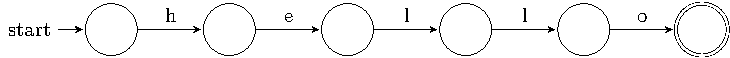
\includegraphics[width=\textwidth]{diagrams/hello-automata.pdf}
      \label{hello-automata}
    \end{figure}

    \marginpar{Here, $\Sigma$ is the alphabet that's being used, so $|\Sigma|$
    is the size of the alphabet, $m$ is the size of the needle, and (you should
    know this one) $\Theta$ is a tight bound on the computation, as opposed to
    $O$, which is an upper bound.}

    The trouble with DFA's is that they are expensive to create (you need a
    method that will ensure you've built a correct DFA), hence the pre-
    processing time for the DFA method is $\Theta(m |\Sigma|)$, which when your
    alphabet is large (like if you're using ASCII, or even Unicode(!)), could be
    significant.

  \item \textbf{Knuth-Morris-Pratt}\\
    The KMP algorithm builds a DFA that will work as above. The main difference
    is that the KMP algorithm also includes how to build the DFA. This is a hard
    algorithm, building a DFA isn't easy! Thankfully, Robert Sedgewick has a fab
    lecture on it that you can watch:
    \url{https://www.youtube.com/watch?v=iZ93Unvxwtw}

\end{description}

\newpage
\section{Code listings}

\marginpar{Can you see a potential security issue with this QuickSort? Take
another look at Section~\ref{QuickSelect} if you can't spot it!}

\lstinputlisting[caption={QuickSort}, label=quicksort]{code/QuickSort.java}
\newpage
\lstinputlisting[caption={MergeSort}, label=mergesort]{code/MergeSort.java}
\newpage
\lstinputlisting[caption={BinarySearch}, label=binarysearch]{code/BinarySearch.java}